\documentclass[12pt]{article}
\usepackage[a4paper, margin=1in]{geometry}
\usepackage{framed}
\usepackage{xcolor}
\usepackage{tikz, pgfplots}
\usepackage[utf8]{inputenc}
\usepackage[T1]{fontenc}
\usepackage[parfill]{parskip}
\usepackage{graphicx}
\graphicspath{ {./images/} }

\raggedright
\definecolor{shadecolor}{RGB}{222,222,222}

\begin{document}

    \catcode`\&=12
    \catcode`\%=12
    \catcode`\#=12
    \catcode`\_=12
    \catcode`\~=12
    \catcode`\^=12

    \title{Project 1 Documentation}
    \author{Sean Bowers}
    \maketitle

    \section*{Compiling}

    This project is writtin in ANSI standard C (C99).

    This project is built with a makefile, which was configured for building on Linux with gcc.
    The project does not have any dependencies (besides the c standard library and math library), so it should work on other platforms.

    To compile, the four .c files in src/ (bitstream.c, crc.c, hamming.c, and main.c) should be compiled with src/ as an include directory.
    This is automatically done with a makefile on Linux systems, and can just be done by running "make" in the root of the project.

    The commands that the makefile runs (on linux) are:

    \textit{Code for part 2:}
    \begin{snugshade*}
    \begin{verbatim}
mkdir -p ./bin
mkdir -p ./obj
gcc -c -o ./obj/bitstream.o src/bitstream.c -Isrc -Wall
gcc -c -o ./obj/crc.o src/crc.c -Isrc -Wall
gcc -c -o ./obj/hamming.o src/hamming.c -Isrc -Wall
gcc -c -o ./obj/main.o src/main.c -Isrc -Wall
gcc -o ./bin/pj1 ./obj/main.o ./obj/bitstream.o \
    ./obj/crc.o ./obj/hamming.o -lm
    \end{verbatim}
    \end{snugshade*}

    \section*{Running}

    This project can be run directly from the makefile, with \verb|make run ARGS="<args>"| where are the arguments to the program specified below.

    The project can also be run directly as a binary after being compiled.
    For example, if the project was compiled to ./bin/pj1, it could be run as \verb|./bin/pj1 <args>|

    The arguments to the program are listed when the program is run with no arguments. The essential arguments are:

    \begin{itemize}
        \item \verb|--part={part}|: specifies which part to run, so for example for part 1.1, the argument would be \verb|--part=1.1|
        \item \verb|--input={input}|: The input to the program
        \item \verb|--generator={generator}|: The generator to use (only for part 2)
        \item \verb|--quiet|: Tells the program to not output any text besides the final output
        \item \verb|--test|: Tells the program to run tests
    \end{itemize}

    \section*{Testing}

    Part 1.1:
    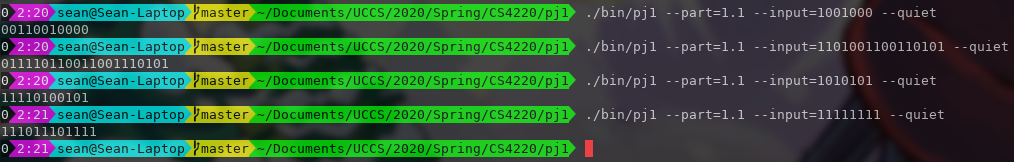
\includegraphics[width=\textwidth]{Tests-Part-1-1}

    Part 1.2:
    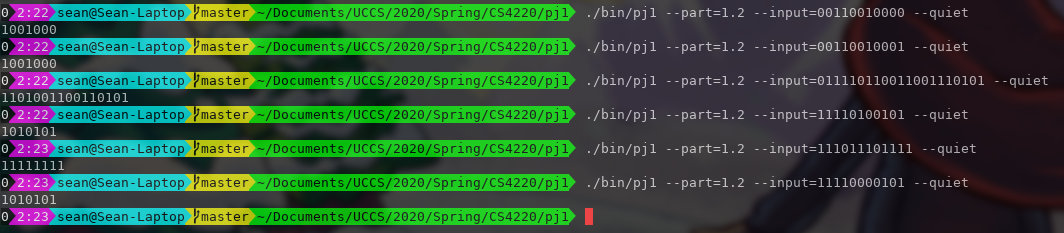
\includegraphics[width=\textwidth]{Tests-Part-1-2}

    Part 2:
    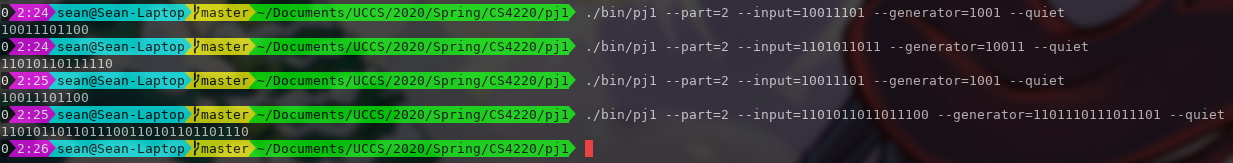
\includegraphics[width=\textwidth]{Tests-Part-2}

\end{document}
